\documentclass{beamer}


\title{kubernetes}
\author{Joris Baiutti}
\institute{Berner Fachhochschule}
\date{\today}

\usepackage{xcolor}
\usepackage{listings}
% Code Listings
\colorlet{punct}{red!60!black}
\definecolor{background}{HTML}{EEEEEE}
\definecolor{delimcode}{RGB}{20,105,176}
\colorlet{numb}{magenta!60!black}
\lstdefinelanguage{json}{
    basicstyle=\normalfont\ttfamily,
    numbers=left,
    numberstyle=\scriptsize,
    stepnumber=1,
    numbersep=8pt,
    showstringspaces=false,
    breaklines=true,
    frame=lines,
    backgroundcolor=\color{background},
    literate=
     *{0}{{{\color{numb}0}}}{1}
      {1}{{{\color{numb}1}}}{1}
      {2}{{{\color{numb}2}}}{1}
      {3}{{{\color{numb}3}}}{1}
      {4}{{{\color{numb}4}}}{1}
      {5}{{{\color{numb}5}}}{1}
      {6}{{{\color{numb}6}}}{1}
      {7}{{{\color{numb}7}}}{1}
      {8}{{{\color{numb}8}}}{1}
      {9}{{{\color{numb}9}}}{1}
      {:}{{{\color{punct}{:}}}}{1}
      {,}{{{\color{punct}{,}}}}{1}
      {\{}{{{\color{delimcode}{\{}}}}{1}
      {\}}{{{\color{delimcode}{\}}}}}{1}
      {[}{{{\color{delimcode}{[}}}}{1}
      {]}{{{\color{delimcode}{]}}}}{1},
}



\begin{document}
\begin{frame}
\titlepage
\end{frame}

\begin{frame}
\frametitle{Classic application deployment process}
\begin{enumerate}
    \item Server staging
    \item Web server installation
    \item install all depencencies
    \item Web Server configuration
    \item install forgotten de
\end{enumerate}
    
\end{frame}

\begin{frame}
\frametitle{What we need to deliver applications and changes fast to the desired systems}
\begin{itemize}
    \item Automated deployment
    \item Versioning
    \item Infrastructure as Code
    \item No dependency hell
    \item Consistent environment (from dev to production)
    \item Immutable
    \item Automated testing
\end{itemize}
\end{frame}

\begin{frame}
\frametitle{What containers can solve}
\begin{itemize}
    \item Isolate applications
    \item Abstraction of resources
    \item Consistent environment
    \item Minimalistic configuration on targed machine
    \item Configuration can be versioned
\end{itemize}
\end{frame}

\begin{frame}
\frametitle{What is a container}
Isolated Artifact which shares the kernel and if possible libraries
    \begin{figure}
        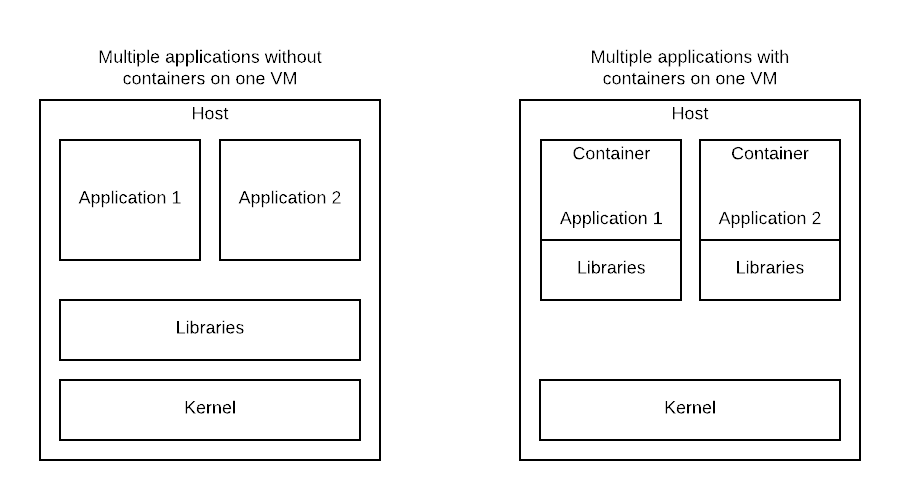
\includegraphics[width=\linewidth]{images/ContainerComparsion.png}
    \end{figure}
\end{frame}

\begin{frame}[fragile]
\frametitle{Example docker file}
\textbf{}
\begin{lstlisting}[language=json,firstnumber=1]
    FROM nginx:1.13.3-alpine
    ## Remove default nginx website
    RUN rm -rf /usr/share/nginx/html/*
    ## From 'builder' stage copy over the artifacts in dist folder to default nginx public folder
    COPY / /usr/share/nginx/html
    CMD ["nginx", "-g", "daemon off;"]
\end{lstlisting}
\end{frame}


\begin{frame}
\frametitle{kubernetes, what is it and why we need it}
\textbf{kubernetes is a container orchestration platform}
\\
    \begin{itemize}
        \item abstraction of infrastructure
        \item desired state
        \item automation
        \item scaling
        \item self healing
    \end{itemize}
\end{frame}



\begin{frame}
\frametitle{How to get kubernetes}
    \begin{itemize}
        \item Minikube
        \item on premise installation
        \begin{itemize}
            \item All pods can communicate with all other pods on all Nodes
            \item All Nodes can communicate with all pods
            \item There is no Network Translation happening (NAT)
        \end{itemize}
        \item cloud platform (Azure, Google, AWS)
    \end{itemize}
    
\end{frame}

\begin{frame}
\frametitle{Overview of kubernetes}
\begin{figure}
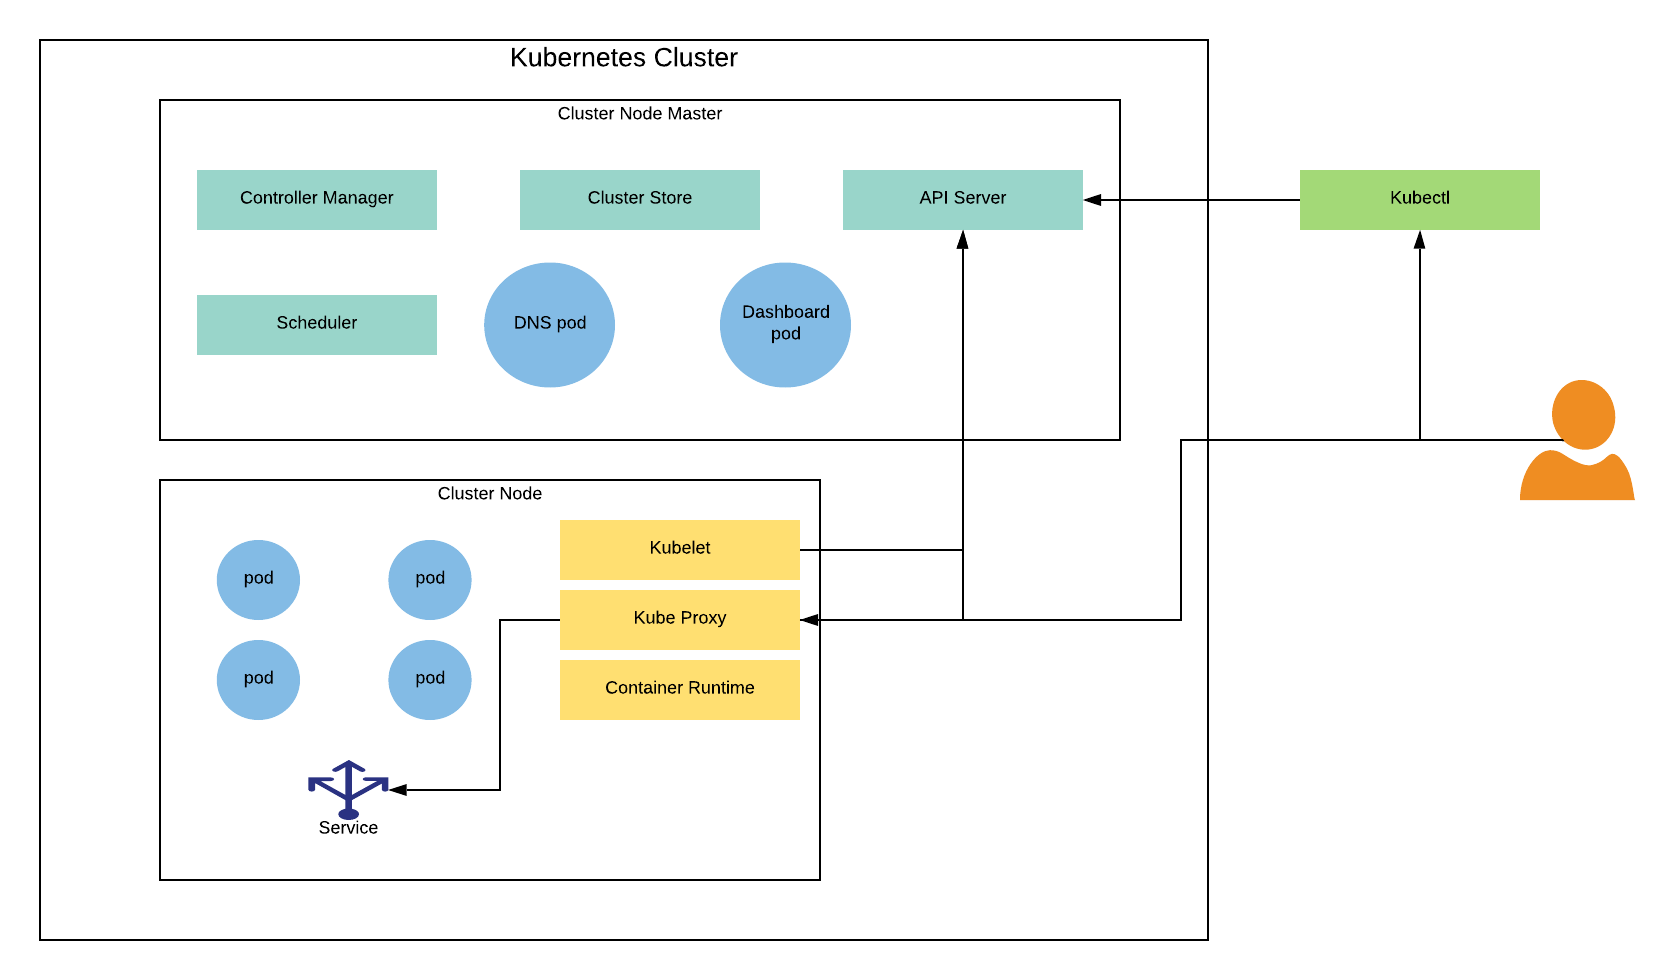
\includegraphics[width=\linewidth]{images/KubernetesOverview.png}
\end{figure}

\end{frame}


\begin{frame}
    \frametitle{Components}
    \begin{columns}
    \column{0.5\textwidth}
    \textbf{Masters}
    \column{0.5\textwidth}
    \textbf{Nodes}
    \end{columns}
    \begin{columns}
    \column{0.5\textwidth}
    \begin{itemize}
        \item API Server
        \item Cluster store
        \item Scheduler
        \item Controller manager
        \item Addon components
    \end{itemize}
    \column{0.5\textwidth}
    \begin{itemize}
        \item Kubelet
        \item Container runtime
        \item Kube proxy
    \end{itemize}
    \end{columns}
\end{frame}


\begin{frame}
\frametitle{What is a pod}
    \begin{figure}
        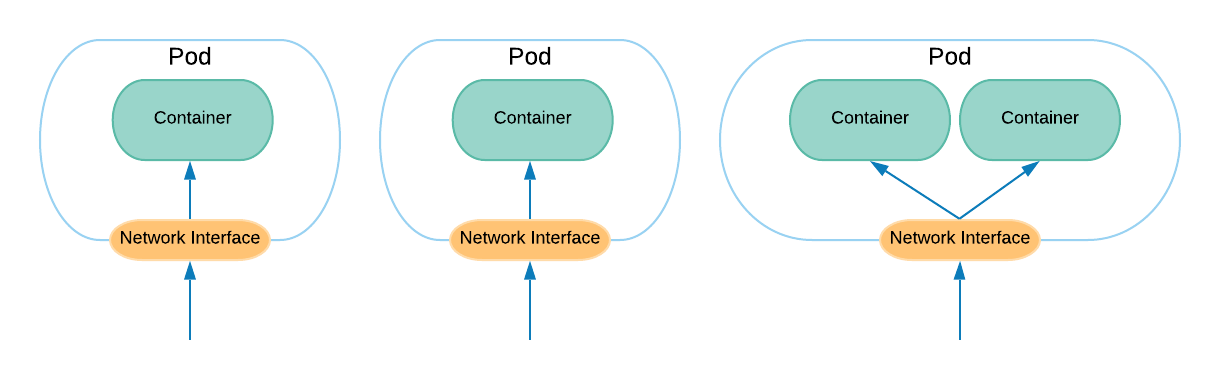
\includegraphics[width=\linewidth]{images/Pods.png}
    \end{figure}
\end{frame}

\begin{frame}
\frametitle{Deployment of pods}
Pods are usually deployed through pod controllers
\begin{itemize}
    \item Replica Set
    \item Deployment
\end{itemize}
\end{frame}



\begin{frame}[fragile]
\frametitle{lifecycle and probes}
\begin{itemize}
    \item ExecAction
    \item TCPSocketAction
    \item HTTPGetAction
\end{itemize}
    \begin{lstlisting}[language=json,firstnumber=1]
    livenessProbe:
          httpGet:
            path: /status/health
            port: 80
          initialDelaySeconds: 90
          timeoutSeconds: 10
\end{lstlisting}
\textbf{Restart policies}
\begin{itemize}
    \item Always
    \item OnFailure
    \item Never
\end{itemize}
\end{frame}


\begin{frame}
\frametitle{Services}
\begin{itemize}
    \item Static endpoint
    \item Mapped to pods
\end{itemize}
    
\end{frame}


\begin{frame}
\frametitle{Demo}
    
\end{frame}

\begin{frame}
\frametitle{Conclusion / Result}
    
\end{frame}

\begin{frame}
\frametitle{Questions?}
    
\end{frame}

\end{document}